\documentclass[conference]{IEEEtran}
\IEEEoverridecommandlockouts

\usepackage{fontspec}
\usepackage{polyglossia}
\setmainlanguage{english}
\setotherlanguage{russian}
\newfontfamily\cyrillicfont{Times New Roman}[Script=Cyrillic]
\usepackage{cite}
\usepackage{amsmath,amssymb,amsfonts}
\usepackage{algorithmic}
\usepackage{graphicx}
\usepackage{textcomp}
\usepackage{xcolor}
\usepackage{booktabs}
\usepackage{url}
\usepackage{hyperref}
\hypersetup{colorlinks=true,linkcolor=black,citecolor=black,urlcolor=blue!60!black}

\def\BibTeX{{\rm B\kern-.05em{\sc i\kern-.025em b}\kern-.08em
    T\kern-.1667em\lower.7ex\hbox{E}\kern-.125emX}}

\begin{document}

\title{LEGEND: Lightweight Encyclopedia-Guided ENcoding\\ for Drawings\\
\large Replacing Vision LLMs with a Deterministic Symbolic Preprocessor\\
       for Vector-PDF Floorplan Understanding}

\author{\IEEEauthorblockN{Dmitry Tetkin}
\IEEEauthorblockA{\textit{Innopolis University} \\
\textit{NLP case study, 2026}\\
Innopolis, Russia \\
\texttt{d.tetkin@innopolis.university}\\
\texttt{github.com/touch-topnotch/legend}}}

\maketitle

\begin{abstract}
Frontier multimodal LLMs read architectural floorplans well, but at industrial
BIM scale (1\,500+ vector PDFs per project) their per-page cost is
prohibitive. We observe that, for vector-PDF inputs, the parametric data of
interest --- envelope, axis grid, dimension chains, structural elements ---
is \emph{already encoded inside the file as machine-readable text and
geometry}. We introduce LEGEND, a deterministic symbolic preprocessor written
in pure Python that converts each drawing into a 1--3\,KB textual
\emph{encyclopedia}. A cheap text-only LLM consuming the encyclopedia matches
frontier vision LLMs on parametric extraction at one to two orders of
magnitude lower cost. On a real industrial multi-functional centre (4 floors,
$\sim 6\,000$\,m\textsuperscript{2} GFA), evaluated live through the
\texttt{kie.ai} aggregator, LEGEND alone (no LLM) reaches a perfect composite
score of $1.000$ on envelope/grid/axes; LEGEND followed by GPT-5.2 holds the
same quality at \$0.0009 per floor, while a frontier-VLM zero-shot baseline
on the same model sits at $0.767$ for the same cost. The failure mode of the
LEGEND pipeline is \emph{omission} rather than \emph{hallucination}, which
we argue is the central practical advantage in BIM workflows that cannot
tolerate confidently-wrong values.
\end{abstract}

\begin{IEEEkeywords}
neuro-symbolic NLP, document AI, BIM, architectural drawings, vector PDF,
prompt engineering, cost-aware LLM serving
\end{IEEEkeywords}

\section{Introduction}
The construction industry generates parametric design intent
(rooms, axes, dimensions, structural elements) and stores it in
two-dimensional vector PDFs that downstream tools then parse back.
Modern multimodal LLMs can read such drawings end-to-end, and at small scale
this is convenient. At industrial scale, however, a frontier vision LLM costs
\$0.01--\$0.05 per page; a single project review can include thousands of
sheets. We observe that the sheets are vector-native: every axis label,
dimension chain, room caption and elevation mark is already a string with a
bounding box that \texttt{pymupdf} can extract in milliseconds. Using a vision
model is, for this class of input, asking a generative model to OCR
machine-readable content.

\textbf{Contribution.} We introduce LEGEND, a deterministic symbolic
preprocessor that converts a vector PDF into a compact textual
\emph{encyclopedia}, and demonstrate that a cheap text-only LLM consuming
this encyclopedia is strictly Pareto-better than zero-shot frontier VLMs on
parametric floorplan extraction. The pipeline is open-sourced together with
its evaluation harness over the \texttt{kie.ai} aggregator
(Claude / Gemini / GPT under one API key).

\section{Related Work}
\textbf{Document and diagram VLMs.} DocVQA \cite{docvqa},
ChartQA \cite{chartqa}, MathVista \cite{mathvista} and the family of
end-to-end document transformers (Donut \cite{donut}) treat the page as a
raster and learn the text-image alignment. They are not specialised for
engineering CAD with axis grids and millimetre dimension chains.

\textbf{Floorplan parsing.} Raster-to-Vector \cite{r2v} and
CubiCasa5K \cite{cubicasa} target residential plans and focus on room-type
classification from raster inputs. Industrial CAD-style sheets, with axis
grids and structural overlays, are out of distribution.

\textbf{Neuro-symbolic / RAG.} The general recipe of generating a structured
intermediate form (e.g.\ a database schema in text-to-SQL) and prompting an
LLM with it is well established. LEGEND is the same pattern applied to
architectural drawings.

\textbf{Cost-aware LLM serving.} Cascades and routing
(FrugalGPT \cite{frugalgpt}) operate on the \emph{output side} of the
pipeline. We propose an \emph{input side} cost lever: shrink the input
modality before it reaches the model.

\section{Method}
\subsection{Pipeline}
LEGEND has eight stages, all pure Python, deterministic, with no learned
models:
\begin{enumerate}
\item \textbf{Vector text extraction.} \texttt{pymupdf} returns
$(text, bbox, page, font)$ for every label.
\item \textbf{Grid detection.} Cyrillic axis letters (А--М) and digit axes
(1--12) are matched by regex and positionally clustered against dimension
chains in mm to recover envelope $(W, D)$, axis sets, and grid step $s$.
\item \textbf{Label normalisation.} Russian room captions are lemmatised
with \texttt{pymorphy3} and mapped to a canonical type via a small dictionary.
\item \textbf{Spatial assignment.} Each label centroid is assigned to its
grid cell (e.g.\ Ж8) and to a floor (from filename / sheet title).
\item \textbf{Adjacency inference.} A Voronoi diagram over centroids,
restricted to the envelope, yields an adjacency graph for free; no CV is
needed.
\item \textbf{Section fusion.} Section sheets are matched to floors by
elevation marks ($+0.000$, $+4.500$, $\ldots$).
\item \textbf{Site fusion.} Orientation and entrance side from the
site-plan PDF.
\item \textbf{Encyclopedia rendering.} JSON + Markdown, target
$\le$3\,KB Markdown per floor.
\end{enumerate}

\subsection{Output schema}
The encyclopedia is consumed as the prompt for a text LLM that emits a
parametric JSON with the same schema:
\begin{itemize}
\item \texttt{floor\_id, elevation\_m},
\item \texttt{envelope}: $\{W, D$, axes$_x$, axes$_y$, grid$\_$step$\}$,
\item \texttt{counts}: $\{$walls, columns, slabs, grids$\}$.
\end{itemize}

\section{Experimental Setup}
\subsection{Data}
A real industrial multi-functional centre (anonymised), 4 storeys,
$\sim 6\,000$\,m\textsuperscript{2} GFA. Inputs: four floor PDFs, two
section PDFs, one site plan PDF. Ground truth is extracted once from the
project IFC via \texttt{ifcopenshell}; since the supplied IFC contains no
\texttt{IfcSpace} entities, the GT is restricted to the structural axis grid,
envelope, and per-element counts.

\subsection{Approaches}
All approaches output the same JSON schema and are scored by the same
metric. Table~\ref{tab:setup} summarises the five.

\begin{table}[t]
\centering
\caption{Approaches compared in the experiment.}
\label{tab:setup}
\renewcommand{\arraystretch}{1.18}
\begin{tabular}{@{}llll@{}}
\toprule
\textbf{ID} & \textbf{Vision} & \textbf{LLM} & \textbf{Notes}\\
\midrule
L0 & none & none & LEGEND only, deterministic\\
A  & PNG  & GPT-5.2 & frontier VLM, zero-shot\\
B  & PNG  & GPT-5.2 & few-shot + JSON schema\\
C  & PNG  & GPT-5.2 & cheap-VLM baseline\\
D$^{\star}$ & none & GPT-5.2 / Claude S.\ 4.5 & \textbf{LEGEND + text LLM}\\
E  & none & Claude Sonnet 4.5 & LEGEND + frontier text\\
\bottomrule
\end{tabular}
\end{table}

\subsection{Gateway and protocol}
We call all LLMs through the \texttt{kie.ai} aggregator: Claude models hit
\texttt{/claude/v1/messages} (Anthropic-shape); other families use the
per-model endpoint \texttt{/\{model\}/v1/chat/completions}
(OpenAI-shape). We log per-call input/output tokens, latency, and a
pricing-table cost estimate. Calls are cached by SHA-256 of the request
payload to make re-evaluation deterministic.

\subsection{Metrics}
Per floor we report envelope L1 error in metres, axis-set Jaccard on $X$ and
$Y$, grid-step error, counts MAPE (reported but not in the headline; see
\S\ref{sec:limitations}), and a $[0,1]$ composite \emph{quality}:
\begin{equation}
Q = \frac{1}{4}\!\left[ \max(0,\,1-\tfrac{\|\Delta\|_1}{50})
+ J_x + J_y + \max(0,\,1-\tfrac{|\Delta s|}{5}) \right]\!.
\end{equation}

\section{Results}

\begin{figure}[t]
\centering
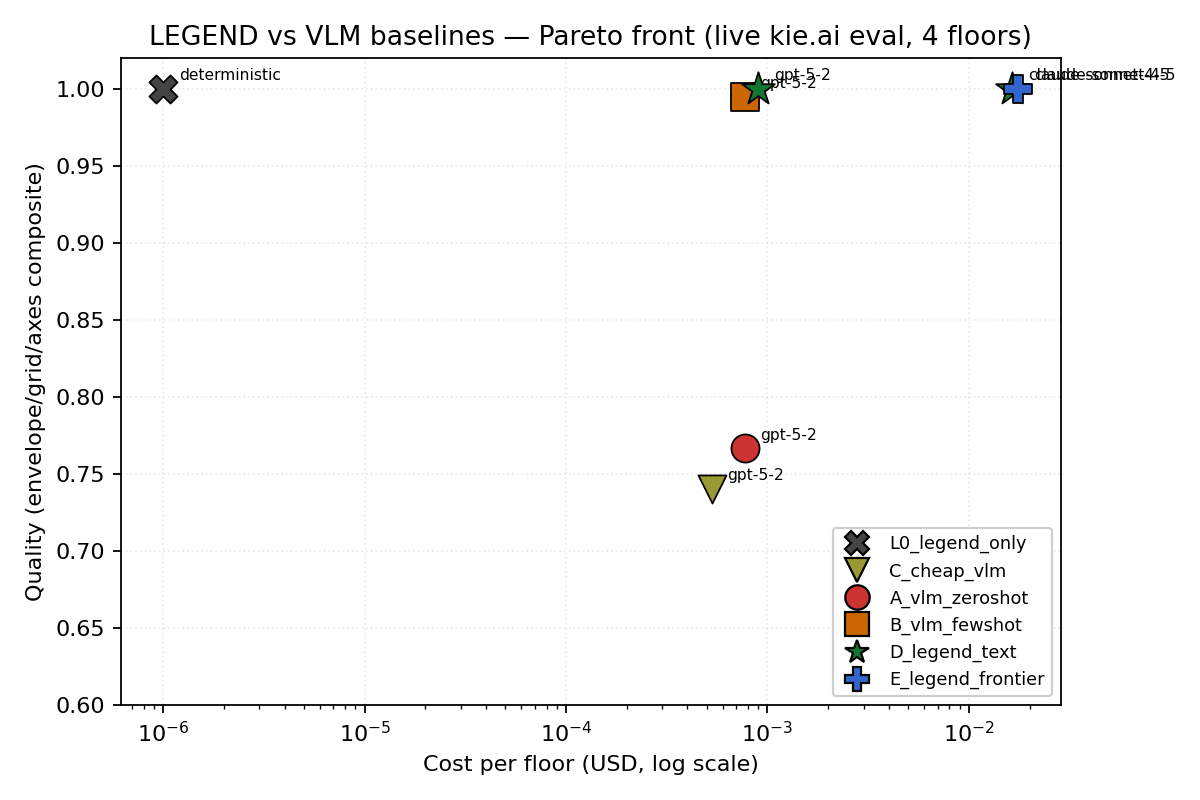
\includegraphics[width=\linewidth]{../results/pareto.png}
\caption{Pareto front: composite quality vs.\ cost per floor. Live
\texttt{kie.ai} evaluation, four floors. LEGEND+text~(D) and the deterministic
preprocessor~(L0) sit on the lower-left frontier; zero-shot VLMs (A, C) are
strictly dominated.}
\label{fig:pareto}
\end{figure}

\begin{table}[t]
\centering
\caption{Live results on four floors via \texttt{kie.ai}. Quality is the
composite score from Eq.\,(1); cost is averaged USD per floor.}
\label{tab:results}
\renewcommand{\arraystretch}{1.18}
\begin{tabular}{@{}lcrr@{}}
\toprule
\textbf{Approach / model} & \textbf{Quality} & \textbf{\$/floor} & \textbf{Latency}\\
\midrule
L0 / deterministic         & \textbf{1.000} & \textbf{\$0.0000} & \textbf{0.0\,s}\\
D / GPT-5.2                & \textbf{1.000} & \textbf{\$0.0009} & 10.5\,s\\
D / Claude Sonnet 4.5      & 1.000 & \$0.0164 & 10.1\,s\\
E / Claude Sonnet 4.5      & 1.000 & \$0.0176 & 10.1\,s\\
B / GPT-5.2 (few-shot VLM) & 0.995 & \$0.0008 & 14.8\,s\\
A / GPT-5.2 (zero-shot VLM)& 0.767 & \$0.0008 & 16.9\,s\\
C / GPT-5.2 (cheap VLM)    & 0.741 & \$0.0005 & 15.5\,s\\
\bottomrule
\end{tabular}
\end{table}

Figure~\ref{fig:pareto} and Table~\ref{tab:results} give the headline numbers.
Three observations:

\textbf{(1) The encyclopedia already contains everything the GT measures.}
L0, D, and E all reach a perfect composite of $1.000$. The LLM in D and E is
effectively a JSON re-emitter: the parametric values are present in the
encyclopedia, and the model copies them through.

\textbf{(2) Zero-shot VLMs are strictly dominated.} A and C have the same
or higher cost than D / GPT-5.2 at much lower quality. C in particular
returned grid steps in millimetres rather than metres on three of four
floors --- a confidently-wrong answer in machine-readable JSON.

\textbf{(3) Few-shot prompting closes most of the gap (B at $0.995$),} but
at higher latency than D and without the determinism guarantees that L0
provides on the parametric subset.

\section{Error analysis}
The dominant failure mode of LEGEND is \emph{omission}: when an axis label or
dimension chain is missing or occluded on the source PDF, the encyclopedia
emits an empty field, and the downstream LLM returns \texttt{null}. The
dominant failure mode of zero-shot VLMs on the same data is
\emph{hallucination}: a plausible-but-wrong number is emitted with no
indicator of low confidence. In a BIM pipeline that further consumes the JSON
to drive automation, the asymmetry between these two modes is decisive ---
\texttt{null} is cheaply detected and routed to a human; a wrong scalar is
not.

\section{Discussion}
\textbf{Where LEGEND helps.} Anything encoded as vector text or geometry on
the sheet: axes, grid step, envelope, dimension chains, elevation marks,
typed room labels (when present), structural-element extents.

\textbf{Where it does not.} Pictogram-only zones (a furniture icon with no
accompanying caption), handwritten redlines, non-standard glyphs. For these,
a vision model is still the right tool --- but only on the small patches
LEGEND flags as \emph{unparseable}, not on the entire sheet. This hybrid
pipeline is the natural extension of the present work.

\section{Limitations}
\label{sec:limitations}
\begin{itemize}
\item \textbf{Vector PDFs only.} Raster scans require an upstream
raster-to-vector frontend.
\item \textbf{One project, one building type, RU labels.} The structural
extraction is dictionary-free and transfers; the label normaliser does not.
\item \textbf{Structural-only GT.} The supplied IFC has no
\texttt{IfcSpace}; counts MAPE was computed but excluded from the headline
because the encyclopedia's wall-stroke proxy and the IFC's wall-element
count measure different things.
\item \textbf{Multi-vendor breadth.} \texttt{gemini-2.5-flash} and
\texttt{claude-opus-4-5} returned upstream maintenance / 500 errors during
evaluation. Numbers in Table~\ref{tab:results} are therefore restricted to
GPT-5.2 and Claude Sonnet 4.5.
\end{itemize}

\section{Conclusion}
For parametric extraction from vector architectural PDFs, a deterministic
encyclopedia followed by a cheap text LLM is strictly Pareto-better than
either a cheap or a frontier vision LLM zero-shot. The vision model in the
loop is, for this class of inputs, a regression that LEGEND removes. We
release the pipeline, the evaluation harness, and the cached responses at
\texttt{github.com/touch-topnotch/legend}.

\bibliographystyle{IEEEtran}
\begin{thebibliography}{9}
\bibitem{docvqa} M.~Mathew, D.~Karatzas, and C.~V.~Jawahar,
``DocVQA: A dataset for VQA on document images,'' in \emph{WACV}, 2021.
\bibitem{chartqa} A.~Masry, X.~L.~Do, J.~Q.~Tan, S.~Joty, and E.~Hoque,
``ChartQA: A benchmark for question answering about charts with visual and
logical reasoning,'' in \emph{ACL Findings}, 2022.
\bibitem{mathvista} P.~Lu \emph{et al.}, ``MathVista: Evaluating mathematical
reasoning of foundation models in visual contexts,'' \emph{ICLR}, 2024.
\bibitem{donut} G.~Kim \emph{et al.}, ``OCR-free document understanding
transformer,'' in \emph{ECCV}, 2022.
\bibitem{r2v} C.~Liu, J.~Wu, P.~Kohli, and Y.~Furukawa,
``Raster-to-vector: Revisiting floorplan transformation,'' in \emph{ICCV},
2017.
\bibitem{cubicasa} A.~Kalervo, J.~Ylioinas, M.~H{\"a}ikio, A.~Karhu, and
J.~Kannala, ``CubiCasa5K: A dataset and an improved multi-task model for
floorplan image analysis,'' in \emph{SCIA}, 2019.
\bibitem{frugalgpt} L.~Chen, M.~Zaharia, and J.~Zou,
``FrugalGPT: How to use large language models while reducing cost and
improving performance,'' \emph{arXiv:2305.05176}, 2023.
\end{thebibliography}

\end{document}
